\chapter{The universal symmetry: the circle}
\label{cha:circle}

An effective principle in mathematics is that when you want to study a certain 
phenomenon you should search for a single type that captures this phenomenon.  
Here are two examples
\begin{enumerate}
\item The contractible type $\bn 1$ has the property that given 
any type $A$ a function $\bn 1\to A$ provides exactly the 
same information as picking an element in $A$.
For, an equivalence from $A$ to $\bn 1\to A$ is provided by
the function $a \mapsto (x \mapsto a)$.
\item The type $\Prop$ of propositions has the property that 
given any type $A$ a function $A\to\Prop$ provides exactly 
the same information as picking a subtype of $A$.
\end{enumerate}
We are interested in symmetries, and so we should search for a type $X$ 
which is so that given \emph{any} type $A$ the type of functions 
$X\to A$ (or $A\to X$, but that's not what we're going to do) 
picks out exactly the symmetries in $A$.  
We will soon see that there is such a type: 
the circle which is built \emph{exactly} so that this 
``universality with respect to symmetries'' holds.  
It may be surprising to see how little it takes to define it; 
especially in hindsight when we eventually discover some of the many uses of the circle.

A symmetry in $A$ is an identification $p:a=_Aa$ for some $a:A$.  
Now, we can take any iteration of $p$ (composing $p$ with itself a number of times), 
and we can consider the inverse $p^{-1}$ and \emph{its} iterations.  
So, by giving one symmetry we at the same time give a lot of symmetries.  
For a particular $p$ it may be that not all of the iterations are different, 
for instance it may be that $p^2=p^0\defequi\refl a$ (like in \cref{xca:C2}), 
or even more dramatic: if  $p=\refl a$, then \emph{all} the iterates of $p$ are equal. 
However, in general we must be prepared that all the powers of $p$ 
(positive, $0$ and negative) are distinct. 
Hence, the circle must have a distinct symmetry for every integer. 
We would have enjoyed defining the integers this way, 
but being that ideological would be somewhat inefficient. 
Hence we give a more hands-on approach defining the circle 
and the integers separately. Thereafter we prove that the type of 
symmetries of the circle is equivalent to the set of integers. 

\section{The circle and its universal property}
\label{sec:S1}

Propositional truncation from \cref{sec:prop-trunc} was
the first \emph{higher inductive type}, that is, an inductive type
with constructors both for elements and for identifications,
we introduced. 
The circle is another example of a higher inductive type,
see Chapter~6 of the HoTT book\footcite{hottbook} for more information.

\begin{definition}
  \label{def:circle}
The circle is a type $\Sc:\UU$ with an element (constructor) $\base : \Sc$ and 
an identification (constructor) ${\Sloop}: \base=\base$. For convenience and
clarity the (higher) induction principle for $\Sc$ is explained
by first stating a recursion principle for $\Sc$.

Let $A$ be a type. In order to define a function $f:\Sc\to A$,
it suffices to give an element $a$ of $A$ together with an
identification $l$ of type $a=a$. The function $f$ defined
by this data satisfies $f(\base)\jdeq a$ and 
the recursion principle provides an (unnamed) element of 
$\ap{f}(\Sloop)=l$.

Let $A(x)$ be a type for every $x:\Sc$. The induction principle of $\Sc$
states that, in order to prove $A(x)$ for every element $x$ of $\Sc$,
it suffices to give an element $a$ of $A(\base)$ together with an
identification $l$ of type $\pathover{a}{A}{\Sloop}{a}$. 
The function $f$ defined by this data satisfies $f(\base)\jdeq a$ and 
the induction principle provides an element of $\apd{f}(\Sloop)=l$.
\end{definition}

Giving $a$ as above is referred to as `the base case', and
giving $l$ as `the loop case'. Given this input data to define
a function $f$ will often be abbreviated by writing
$f(\base)\defeq a$ and $f(\Sloop)\defis l$.

The following result states that any function from the circle exactly 
picks out an element and a symmetry of that element.
This is a ``universal property'' of the circle.

\begin{lemma}\label{lem:freeloopspace}
For all types $A$, the evaluation function 
\[
\ev_A : (\Sc\to A)\to \sum_{a:A}(a=_Aa)\text{~defined by~} 
\ev_A(g)\defeq (g(\base),g(\Sloop))
\]
is an equivalence, with inverse $\el_A$ defined by the recursion principle.  
In particular, if $a:A$, the function $((\Sc,\base)\to_* (A,a))\to (a=_Aa)$
sending $(g,p)$ to $p^{-1}\cdot g(\Sloop)\cdot p$ is an equivalence.
\end{lemma}
\begin{proof}
Fix $A:\UU$. We apply \cref{lem:weq-iso}. 
For all $a:A$ and $l:a=a$ we have $\ev(\el(a,l))=(a,l)$
by the recursion principle. It remains to prove
$\el(\ev(f))=f$ for all $f:\Sc\to A$. This will follow
from the following more general result. Assume 
$p: f(\base)= g(\base)$ and $q: f(\Sloop) = p^{-1}\cdot g(\Sloop)\cdot p$.
We show $f=g$, for which it suffices to prove by circle induction
that $P(x)\defeq(f(x)=g(x))$ for all $x:\Sc$.
For the base case we take $p$.
The loop case reduces to $\trp[P]{\Sloop}(p)=p$ by \cref{def:pathover-trp}.
By \cref{lem:trp-in-fx=Ygx} we have 
$\trp[P]{\Sloop}(p)=g(\Sloop)\cdot p \cdot f(\Sloop)^{-1}$. 
By $q$ we have $g(\Sloop) = p\cdot f(\Sloop) \cdot p^{-1}$.
Hence $\trp[P]{\Sloop}(p)=p$ by easy calculation.
Using \cref{lem:isEq-pair=} we can phrase the result
as: if $\ev(f)=\ev(g)$, then  $f=g$.

Now we get $\el(\ev(f))=f$, as
$\ev(\el(\ev(f)))=(f(\base),f(\Sloop))\jdeq\ev(f)$ with $p\defeq\refl{f(\base)}$
and $q$ coming from the induction principle.
\end{proof}

{\color{blue}
The above proof is a function $e$ of type $\prod_{A:\UU} \isEq(\ev_A)$.
This means that for all $A:\UU$, $a:A$ and $p:a=a$, 
$e(A,a,p)$ is a proof that $\ev_A^{-1}(a,p)$ is contractible. Hence 
%$\fst(e(A,a,p)): \sum_{f:\Sc\to A}(a,p)=\ev_A(f)$ is the center of contraction, and 
$\fst(\fst(e(A,a,p))):\Sc\to A$. 
We denote $\fst(\fst(e(A,a,p)))$ by $\ve_A(a,p)$. When we specify a function
$f:\Sc\to A$ by $f(\base)\defeq a$ and $f(\Sloop)\defis p$ we mean
$f\defeq\ve_A(a,p)$.
}

\begin{remark}\label{rem:dep-univ-prop-circle}
By almost the same argument as for \cref{lem:freeloopspace}
one can obtain the dependent universal property of the circle.
Given a type family $A:\Sc\to\UU$, the evaluation function
$(\prod_{x:\Sc} A(x))\to \sum_{a:A(\base)}(\pathover a A {\Sloop} a)$
is an equivalence.
\end{remark}


\begin{remark}
A function $f:\Sc\to A$ is often called a \emph{loop} in $A$, 
the picture being that $f$ throws $\Sloop:\base=\base$ as a lasso in the type $A$.

  Under univalence, so that $a=_Aa$ is identified with the pointed functions 
from the circle, this allows for a very graphic interpretation of the 
symmetries in $a=_Aa$: they are all in the image of a function $g$ from 
the circle: they are loops in the type $A$ starting and ending at $a$! ((picture!!))
\end{remark}

\begin{lemma}\label{lem:circleisconnected}
  The circle is connected.
\end{lemma}
\begin{proof}
We show $\Trunc{\base=z}$ for all $z:\Sc$ by circle induction
as in \cref{def:circle}.
For the base case we take $\trunc{\refl{\base}}$.
The loop case is immediate as $\Trunc{\base=\base}$ is a proposition.
\end{proof}

In the proof above, the propositional truncation coming 
from the definition of connectedness is essential.
If this truncation were removed we wouldn't know what to do in
the induction step (actually, ${\base=z}$ for all $z:\Sc$ contradicts UA).
This said, the family $R:\Sc\to\UU$ with $R(z)\defequi (\base=z)$ is extremely 
important for other purposes. We will call it in \cref{def:universalcover} the 
``universal \covering'' of the circle and is the key tool in proving that 
the set of integers and the symmetries of the circle coincide.
By the ``symmetries of the circle'' we mean the elements of $\base=_{\Sc}\base$,
not $\Sc=_{\UU}\Sc$. The latter type is equivalent to $\Sc\amalg\Sc$,
as follows from \cref{xca:S1=S1-components} and \cref{{xca:(S1->S1)_(f)-eqv-S1}}.



In order to do this we should properly define the set of integers 
and explore the concept of \coverings.

\section{The integers}
\label{sec:integers}

We define the type of integers in one of the many possible ways.

\begin{definition}\label{def:zet}
  Let $\zet$ be the inductive type with the following three
  constructors:
\begin{enumerate}
\item $z_0: \zet$ for the integer number zero,
$0 \defeq z_0$
\item $pos: \NN \to \zet$ for positive numbers,
$1 \defeq pos(0),\ldots$
\item $neg: \NN \to \zet$ for negative numbers, 
$-1 \defeq neg(0),\ldots$
\end{enumerate}
Like any other inductive type, the type $\zet$ comes with an
induction principle. Let $T(z)$ be a family of types indexed by $z:\zet$.
In order to construct an element $f(z)$ of $T(z)$ for all $z:\zet$,
it suffices to give $f(0): T(0)$ and to give functions $g$ and $h$ such
that $g(n): T(pos(n))$ and $h(n): T(neg(n))$ for all $n:\NN$.
Here $g$ and $h$ can be defined by induction on $n:\NN$.

The \emph{embedding} function $i:\NN\to\zet$ is defined by induction,
setting $i(0)\defeq z_0$, $i(S(n))\defeq pos(n)$.
Like the type $\NN$, the type $\zet$ is a set with decidable equality
and ordering relations,
and we denote its elements often in the usual way as $\ldots,-1,0,1,\ldots$.

One well-known equivalence is \emph{negation} ${-}:\zet\to\zet$, 
also called \emph{complement}, inductively defined by setting 
$-z_0\defeq z_0$, 
$-pos(n)\defeq neg(n)$, 
$-neg(n)\defeq pos(n)$.
Negation is its own inverse.

The \emph{successor} function $s:\zet\to\zet$ is defined inductively setting 
$s(z_0)\defeq pos(0)$, 
$s(pos(n))\defeq pos(S(n))$,
$s(neg(n))\defeq -i(n)$. For example, we have
$s(-1)\jdeq s(neg(0))\jdeq -i(0) \jdeq z_0 \jdeq 0$.
By induction on $n:\NN$ one proves $s(i(n))=i(S(n))$, 
so that one can say that $s$ extends $S$
on the $i$-image of $\NN$. 

The successor function $s$ is an equivalence.
It is instructive to depict iterating $s$ in both directions as 
a doubly infinite sequence containing all integers:
\[
\ldots \mapsto neg(1) \mapsto neg(0) \mapsto z_0 \mapsto pos(0) \mapsto pos(1) \mapsto \ldots
\]

The inverse $s^{-1}$ of $s$ is called the \emph{predecessor} function.
We recall the $n$-fold iteration $s^n$ defined earlier;
the $n$-fold iteration of $s^{-1}$ will be denoted by $s^{-n}$.

Addition of integers is defined inductively by setting
$z + z_0\defeq z$, 
$z + pos(n)\defeq s^{n+1}(z)$, 
$z + neg(n)\defeq s^{-(n+1)}(z)$.
Again, addition extends $+$ on the $i$-image of $\NN$,
see \cref{xca:addition-on-Z-and-N}. 
From addition and unary $-$ one can define a binary
\emph{substraction} function setting $z-y \defeq z+(-y)$.
\end{definition}

\begin{xca}\label{xca:addition-on-Z-and-N}
Show that $i(n+m)=i(n)+i(m)$ for all $n,m:\NN$.
\end{xca}

Ordering relations $<$ and $\leq$ on $\zet$ are easily defined
and shown to extend those on $\NN$.

Recall the induction principle for $\zet$ in \cref{def:zet} above.
Instead of defining $g$ and $h$ explicitly, we will often
define $g'$ and $h'$ such that $g'(z): T(z)\to T(z+1)$ 
for all $z:\zet$ with $z\geq 0$, and $h'(z): T(z)\to T(z-1)$ 
for all $z:\zet$ with $z\leq 0$. The function $f$ defined by 
satisfies $f(z+1)\jdeq g'(z,f(z))$ for all $z\geq 0$,
and $f(z-1)\jdeq h'(z,f(z))$ for all $z\leq 0$.

\begin{xca}\label{xca:commutative-add-Z}
Show that $n+m = m+n$ for all $n,m:\zet$.  
\end{xca}


\section{\Coverings}
\label{sec:covering}

As mentioned earlier, it is possible to define the integers as the
type $\base=_{S^1}\base$ of symmetries of the circle.
Our investigation of $\base=_{S^1}\base$ will use the concept of \coverings. 
Since we are going to return to this concept several times, 
we take the time for a fuller treatment before we continue with
proving the equivalence of $\base=_{S^1}\base$ and $\zet$.

\begin{definition}\label{def:covering}
A \emph{\covering} over a type $B$ 
is a map $f:A\to B$ such that for each $b:B$ the preimage $f^{-1}(b)$ is a set.
We say that a \covering $f:A\to B$ over $B$ is
\begin{itemize}
\item \emph{connected}\index{connected \covering} if $A$ is connected, 
\item \emph{universal}\index{universal \covering} if $A$ and all 
the identity types $a=_Aa$ (for $a:A$) are connected, 
\item \emph{finite}\index{finite \covering} if all preimages are finite sets,
\item \emph{decidable}\index{decidable \covering} if all preimages are decidable sets.
\end{itemize}
If $B$ is a pointed type, a \emph{pointed} \covering is a pointed map $f:A\to_*B$ such that, when forgetting the points, $f_\div:A_\div\to B_\div$ is a \covering. Here we only
require $A$ to be a pointed type. Of course we do get the base point of $A$ in the 
preimage of the base point of $B$, but we do not require the preimages of $f_\div$
to be pointed types.
\end{definition}
With a formula, given a type $B$, the type of \coverings over $B$ is
\[
\SetBundle(B) \defeq \sum_{A:\UU}\sum_{f:A\to B}\prod_{b:B}\isset(f^{-1}(b)),
\]
with variations according to the flavor.

Recall the equivalence in \cref{lem:Prop-Set-pointed-families}\ref{lem:Set-families}
between the type $B\to\Set$ of families of sets indexed by $B$, and the type
of \coverings over $B$ given above.
We shall frequently use this equivalence, even without explicit mention.

\begin{lemma}\label{lem:setbundle-is-groupoid}
For any type $B$, $\SetBundle(B)$ is a groupoid.
\end{lemma}
\begin{proof}
By \cref{lem:Set-is-groupoid} we have that $\Set$ is a groupoid, 
and hence $B\to\Set$ is a groupoid by \cref{lem:level-n-utils}\ref{level-n-utils-codom}.
Moreover, by \cref{cor:subtype-same-level}, all variations in \cref{def:covering}
defined by a predicate are groupoids as well.
\end{proof}
One notable exception to the above lemma is the type of \emph{pointed} \coverings:
a point is extra structure, not just a property.

We should notice that the notion of a \covering is just one step up from the notion of an
injection (a map such that all the preimages are propositions -- 
following the logic, injections perhaps ought to be called ``proposition bundles''). 
The formulation we give is not the only one and for some purposes a formulation
based on $B\to\Set$ is more convenient.

\begin{xca}\label{xca:constant-cover}
Let $A$ and $B$ be types, and let $b$ be an element of $B$.
Show that the function that is constant $b$ is a \covering
if and only if both $A$ and $b=b$ are sets. SPLIT AND EXTEND WITH COMPOSITION
\end{xca}

Figure~\ref{fig:covering} visualizes two examples of \coverings over the circle.  
Consider the picture on the left first.  
If we let $b$ be the element on the circle marked at the bottom left hand side, 
then the preimage $f^{-1}(b)$ is marked by the the two dots in $A$ straight above $b$, 
so that in this case each preimage contains two points (is \emph{merely equal} to $\bn 2$).  
However, $A$ is not the constant family, like $A'$ depicted on the right, since 
$A'=\sum_{z:\Sc}\bn 2=\Sc\times\bn 2=\Sc+\Sc$ is not connected.  
Obviously something way more fascinating is going on.
(In fact the \covering on the left is given by $\ve(\bool,ua(\twist))$,
see \cref{xca:C2} and \cref{lem:freeloopspace}).

\begin{figure}[hbt]
  \centering
  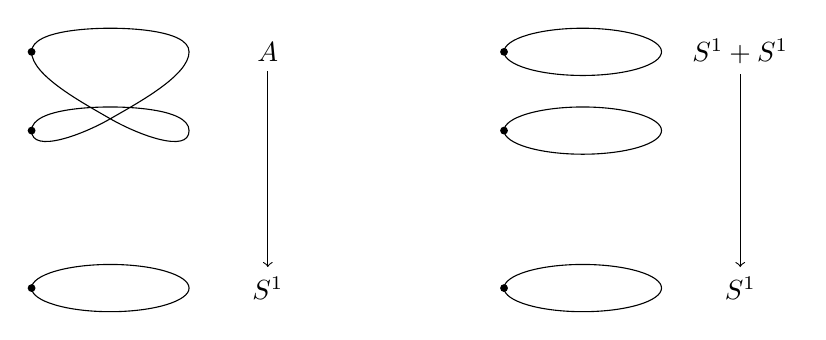
\begin{tikzpicture}
    \node (A) at (2,1) {$A$};
    \node (B) at (2,-2) {$S^1$};
    \draw[->] (A) -- node[auto] {$$} (B);
    \draw (0,-2) ellipse (1 and .3);
    \draw (-1,0)
    .. controls ++( 90:-.3) and ++(210: .4) .. (0,0.15)
    .. controls ++(210:-.4) and ++(270: .3) .. (1,1)
    .. controls ++(270:-.3) and ++(  0: .1) .. (0,1.3)
    .. controls ++(  0:-.1) and ++( 90: .3) .. (-1,1)
    .. controls ++( 90:-.3) and ++(150: .4) .. (0,0.15)
    .. controls ++(150:-.4) and ++(270: .3) .. (1,0)
    .. controls ++(270:-.3) and ++(  0: .1) .. (0,0.3)
    .. controls ++(  0:-.1) and ++( 90: .3) .. (-1,0);
    \node[fill,circle,inner sep=1pt] at (-1,-2) {};
    \node[fill,circle,inner sep=1pt] at (-1,0) {};
    \node[fill,circle,inner sep=1pt] at (-1,1) {};
%    \node (L) at (1,-3) {(left)};
    \begin{scope}[xshift=6cm]
    \node (At) at (2,1) {$S^1+S^1$};
    \node (Bt) at (2,-2) {$S^1$};
    \draw[->] (At) -- node[auto] {$$} (Bt);
    \draw (0,-2) ellipse (1 and .3);
    \draw (0,0) ellipse (1 and .3);
    \draw (0,1) ellipse (1 and .3);
    \node[fill,circle,inner sep=1pt] at (-1,-2) {};
    \node[fill,circle,inner sep=1pt] at (-1,0) {};
    \node[fill,circle,inner sep=1pt] at (-1,1) {};
%    \node (Lt) at (1,-3) {(right)};
    \end{scope}
  \end{tikzpicture}
  \caption{A visualization of two \coverings over the circle}
  \label{fig:covering}
\end{figure}

\begin{remark}
  It \emph{is} possible to misunderstand what a ``connected \covering'' is: 
the other interpretation ``all the preimages are connected'' simply 
would give us an equivalence (since connected sets are contractible),
and this is \emph{not} what is intended. (Equivalences are \coverings, 
but not necessarily connected \coverings and connected \coverings are not neccesarily equivalences.)  

Likewise, for the other qualifications; for instance in a ``finite covering'' $f:A\to B$, 
the type $A$ is usually \emph{not} a finite set. 

We trust the reader to keep our definitions in mind and not the other interpretations.
\end{remark}


\begin{remark}
  \Coverings are closely related to a concept from topology called ``covering space'' 
(or any variant of this concept, including Galois theory) and from algebra as sheaves (of sets).  
Either way, the concept is useful because it singles out the (sub)symmetries.  
\end{remark}

\begin{example}\label{xca:coveringsofS1}
Let us consider \coverings over the circle, most conveniently 
for the moment in the guise of families 
$$E:\Sc\to\Set.$$
By circle induction, giving such an $E$ is the same as 
specifying a set $E(\base)$ and a symmetry $E(\Sloop):E(\base)=E(\base)$.  
Said more concisely in terms of \cref{lem:freeloopspace}, 
the type of \coverings over the circle is equivalent to 
$$\sum_{X:\Set}(X=X).$$
\end{example}
A particularly important example is the following:
\begin{definition}\label{def:RtoS1}
Define $R:\Sc\to\UU$ by circle induction by setting 
$R(\base)\defeq\zet$ and $R(\Sloop)\defis \etop{s}$.
Since $\zet$ is a set, and being a set is a proposition,
one can prove by circle induction that $R(z)$ is a set for all $z:\Sc$.
(Abusing notation we also write $R:\Sc\to\Set$.) Now define
$$\RR\defeq\sum_{z:\Sc}R(z)$$
and let the first projection denoted by
$$\exp:\RR\to \Sc$$
be the \emph{exponential \covering of the circle}.
\end{definition}

\begin{remark}
  \label{rem:expforreal}
  The reason for the name $\exp:\RR\to \Sc$ comes from the following visualization.   
If $x$ is a real number, then the complex exponentiation 
$e^{2\pi i x}=\cos(2\pi x)+i\sin(2\pi x)$ has absolute value $1$ and 
so defines a continuous function from the real numbers to the unit circle.  
Choosing any point $z$ on the unit circle, we see that the preimage of $z$ under 
the exponential function is a shifted copy of the integers inside the reals. 
 
This connection between the integers and the unit circle is precisely captured in 
a form that we can take further by the \covering $\exp:\RR\to \Sc$.
\end{remark}

We already defined a \covering $f:A\to B$ to be universal if $A$ is connected
and all $a=_A a$ (for $a:A$) are connected. 
If moreover $B$ is a pointed, connected groupoid we shall argue that
we actually can speak of \emph{the} universal \covering.

Recall \cref{cor:fib-vs-path} stating that all the fibers of a map $f:A\to B$ 
are sets if and only if each 
\[
\ap{f}: (a=a')\to (f(a)=f(a'))
\]
is an injection. 
Assume $f:A\to B$ is a universal \covering and $B$ is a groupoid.
We prove that $A$ is contractible. 
Being contractible is a proposition, so we may assume 
we have an element $a$ of $A$ since $A$ is connected. 
By \cref{xca:connected-trivia} and \ref{xca:component-connected} 
it suffices to prove that $a=a$ is contractible.
By \cref{xca:prop-set-trivia}, using that $a=a$ is connected,
it suffices to show that $a=a$ is a set.
Using that $\ap{f}$ is an injection, we can apply the remark after
\cref{lem:sum-of-fibers} and obtain that $a=a$ is a set since
$f(a)=f(a)$ is a set, since $B$ is a groupoid.
This completes the proof that $A$ is contractible.

Now assume $(B,b_0)$ is a pointed connected groupoid and $f:A\to B$
a universal \covering. Since $A$ and $\sum_{b:B}(b_0=_Bb)$ are both
contractible, and $B$ is connected, we have
$\Trunc{(A,f)=(\sum_{b:B}(b_0=_Bb),\fst)}$. 
Hence if $(B,b_0)$ is a pointed connected groupoid, all
universal \coverings are merely equal to a canonical one. 
This justifies the following definition.
\begin{definition}
  \label{def:universalcover}
  Let $(B,b_0)$ be a pointed connected groupoid.  
The \emph{universal \covering} of $B$ is the \covering of $B$ given by the family of sets 
  $$\uc{b_0}:B\to\Set,\quad \uc{b_0}(b)\defequi (b_0=_Bb),$$
or alternatively as the first projection from $\uc{b_0}B\defequi\sum_{b:B}(b_0=_Bb)$ to $B$. 
\end{definition}
Note that $(b_0=_B b)$ is a family of \emph{sets} exactly when $B$ is a groupoid.
The type family $(b_0=_B b)$ is also important if $B$ is not a groupoid,
but is then not a \emph{set} bundle.
However, we have \cref{lem:thepathspaceiscontractible} for any type $B$.

\begin{remark}
  What's so ``universal'' about this?
The universal \covering over the pointed connected groupoid $(B,b_0)$ coincides with the constant function $c_{b_0}:\bn 1\to B$ (with value $b_0$), and seems like an unnecessary complicated representation were it not for the manifold practical value of the formulation that we've given.  
In particular, we recognize the set of symmetries $b_0=_Bb_0$ as the preimage of $b_0$ under the first projection from $\uc{b_0}B$ to $B$; ultimately this will show that the study of symmetries coincides with the study of the universal \covering.

The first instance of this comes already in the next section, where we show in \cref{cor:S1groupoid} that the symmetries of the circle are given by the set of integers $\zet$ by showing that the universal \covering and the exponential \covering (\cref{def:RtoS1}) of the circle coincide.

That said, one way to see that the constant function $c_{b_0}:\bn 1\to B$
\emph{does} deserve the label universal is the following. 
Given any function $f:A\to B$ and $(a_0,p): f^{-1}(b_0)$, 
we get a function $c_{a_0}:\bn 1\to A$, and $p:b_0=f(a_0)$ gives rise to
an element in $c_{b_0}=_{\bn 1\to B}f\, c_{a_0}$.  
In other words, any such $f$ is ``a factor of $c_{b_0}$''.  
Note, however, that this depends on $f^{-1}(b_0)$ being non-empty
(classically, this is often demanded of a covering, which distinguishes it from our \coverings), 
and the factorization depends on the element $(a_0,p)$ used. 
\end{remark}



\section{The symmetries of the circle}
\label{sec:symcirc}

With the set $\zet$ of integers \emph{defined} as in \cref{sec:integers}, 
we will now \emph{prove} that $\zet$ is equivalent to the type 
$\base=_{\Sc}\base$, and that under this equivalence $0:\zet$ corresponds to 
$\refl{\base}:\base=\base$, and $1$ to $\Sloop$, and $-1$ to $\Sloop^{-1}$. 
More generally, the successor $\etop{s}:\zet=\zet$ corresponds to composition with $\Sloop$
and the predecessor corresponds to composition with $\Sloop^{-1}$.

The first step is to prove that the exponential \covering \cref{def:RtoS1} 
is equal to the universal \covering in \cref{def:universalcover}, 
\ie we prove that the family 
\[
R: \Sc\to\UU,\qquad R(\base)\defeq\zet,\, R(\Sloop)\defis \etop{s}
\]
is equal to the family
\[
\uc{\base}:\Sc\to\UU,\qquad \uc{\base}(z)\defeq (\base=z).
\]
What does it mean for the families $\uc{\base}$ and $R$ to be equal?
Type families are a special case of functions. 
Function extensionality reduces the question to pointwise equality
of $\uc{\base}$ and $R$ as functions.
Using univalence, it suffices to give
an equivalence from $\uc{\base}(z)$ to $R(z)$ for every $z:\Sc$,
that is, recalling \cref{def:function-type-families}
an equivalence $f: \uc{\base}\to R$. We will use
\cref{lem:weq-iso}, so will also define $g: R\to\uc{\base}$.

We first recall from \cref{sec:heavy-transport} how 
transport behaves in families of function types.  
Given a type $A$ and two type families $P,Q:A\to\UU$,  
transport along $p:a=_Aa'$ of $h:P(a)\to Q(a)$ is $Q(p)\,h\,P(p)^{-1}:P(a')=Q(a')$.
In a picture
\[
\xymatrix{
a\ar@{=}[d]^{p}_\downarrow &&
P(a)\ar[rr]^{h}\ar@{=}[d]^{P(p)}_\downarrow&&
Q(a)\ar@{=}[d]^{Q(p)}_\downarrow\\
a'&&P(a')&&\,Q(a').}
\]
If $A$ is $\Sc$, then the induction principle for the circle says 
that giving an $h(z):P(z)\to Q(z)$ for all $z:\Sc$ is the same as 
specifying an $h(\base):P(\base)=Q(\base)$ and an identity 
$f(\Sloop):Q(\Sloop)\,h(\base)\,P(\Sloop)^{-1}=_{P(\base)\to Q(\base)}h(\base)$,
\ie   a witness that the composites in 
$$\xymatrix{
  P(\base)\ar[rr]^{h(\base)}\ar@{=}[d]^{P(\Sloop)}_\downarrow
 &&Q(\base)\ar@{=}[d]^{Q(\Sloop)}_\downarrow\\
  P(\base)\ar[rr]^{h(\base)}&&\,Q(\base)}
$$
are equal. If $P,Q$ are families of sets, 
then the type of $h(\Sloop)$ is a proposition.

We now define $f: \uc{\base}\to R$ and $g: R\to\uc{\base}$ that will turn out to
give inverse equivalences between $\uc{\base}(z)$ and $R(z)$, for each $z:\Sc$.

\begin{definition}
  \label{def:fPtoR}
  The function $f:\prod_{z:\Sc}(\uc{\base}(z)\to R(z))$ is defined by transport: $f(z)(p)\defequi\trp[R]{p}(0)$.
\end{definition}

In Figure~\ref{fig:transportalongloop}, the transport in the definition
above has been visualised for $p={\Sloop^n}$, $n=-2,-1,0,1,2$.

\begin{figure}[h]
\vspace{1in}
\DELETE% comment this line out to include slow picture
{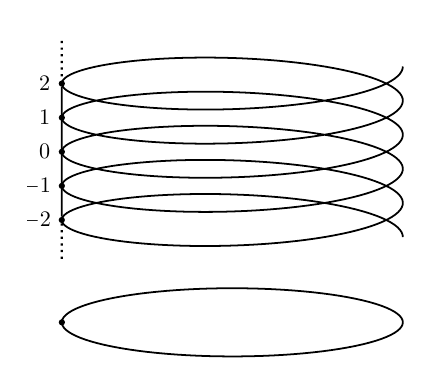
\begin{tikzpicture}[scale=0.8]
\begin{axis}[axis lines=none,line width=1pt, axis equal image]

\node at (-10,13) () {$\zet$}; %CUTOFF FOR UNKNOWN REASON
\node [] at (-10,12) (A) {};

\addplot[domain=0:10*pi,samples=500,black,no marks,thick] %500 samples slow
({10*cos(deg(x))}, % x-coordinate
{2*sin(deg(x)) + x/pi}) % y-coordinate
node [circle,scale=0.3,fill,pos=0.9] (B) {} % point (A)
node [circle,scale=0.3,fill,pos=0.7] {} % point (A)
node [circle,scale=0.3,fill,pos=0.5] {} %
node [circle,scale=0.3,fill,pos=0.3] {} % 
node [circle,scale=0.3,fill,pos=0.1] (C) {}; %

\node at (-11,9) () {$2$};
\node at (-11,7) () {$1$};
\node at (-11,5) () {$0$};
\node at (-11,3) () {$-1\;\;\,$};
\node at (-11,1) () {$-2\;\;\,$};

\node [] at (-10,-2) (D) {};
\node at (0,-5) () {$\Sc$};
\node at (9,-5) () {$\Sloop$};

\addplot[domain=0:2*pi,samples=100,black,no marks,thick] %500 samples slow
({10*cos(deg(x))}, % x-coordinate
{2*sin(deg(x))-5}) % y-coordinate
node [circle,scale=0.3,fill,pos=0.5] (E) {}; % point (D)


\draw[dotted] (A)--(B);
\draw[thick] (B)--(C);
\draw[dotted] (C)--(D);

\end{axis}
\end{tikzpicture}}%DELETE
\caption{Transport in the family $R$}
\label{fig:transportalongloop}
\end{figure}

\begin{lemma}\label{lem:windingnumber}
For $f$ as in \cref{def:fPtoR} we have $f(\base)(\Sloop^n)=n$ for all $n:\zet$.
\end{lemma}
\begin{proof}
By induction on $n:\zet$.  In the base case $n=0$ we have
$f(\base)(\Sloop^0)\defeq f(\refl\base)\defeq 0$.
For $n=s(m)$ with $m:\NN$ we have
\begin{align*}
  f(\base)(\Sloop^{s(m)})&\jdeq\trp[R]{\Sloop^{s(m)}}(0)\\
  &=\trp[R]{\Sloop \Sloop^{m}}(0)\\
  &=\trp[R]{\Sloop}(\trp[R]{\Sloop^m}(0))\\
  &\jdeq \trp[R]{\Sloop}(f(\base)(\Sloop^{m}))\\
  &= s(f(\base)(\Sloop^{m})).
\end{align*}
The last step follows from $\etop{s}=R(\Sloop)$ 
and $s=\trp[\id_\UU]{\etop{s}}$, see \cref{def:univalence},
and hence $s=\trp[\id_\UU]{R(\Sloop)}=\trp[\id_\UU R]{\Sloop}=\trp[R]{\Sloop}$. 
This completes the induction step for positive $n$.
For negative $n$ the proof is similar.
\end{proof}

In the definition of the second map, 
take into account that $R(\base)\jdeq \zet$ and $\uc{\base}(\base) \jdeq (\base=\base)$.

\begin{definition}\label{def:gRtoP}
The function $g:\prod_{z:\Sc}(R(z)\to \uc{\base}(z))$ is 
defined by circle induction: 
\[
g(\base)\defeq {\Sloop^{-}}:\zet\to(\base=\base) : n \mapsto {\Sloop^n}
\]
and 
\[
g(\Sloop): \uc{\base}(\Sloop)\, g(\base)\,R(\Sloop)^{-1}=_{\zet\to (\base=\base)} g(\base).
\]
So far we have only given the type of $g(\Sloop)$. By definition, $R(\Sloop)$ is $s$
and $\uc{\base}(\Sloop)$ is composition with $\Sloop$.
In a picture, $g(\Sloop)$ should prove that it does not matter what 
path you take around the square
$$\xymatrix{\zet\ar[rr]^{\Sloop^-}\ar@{=}[d]^s_\downarrow
 &&(\base=\base)\ar@{=}[d]^{\Sloop\cdot\_}_\downarrow\\
  \zet\ar[rr]^{\Sloop^-}&&\,(\base=\base).}
$$
This follows by a simple calculation: ${\Sloop\,\Sloop^{n-1}} = {\Sloop^n}$, 
for all $n:\zet$. 
\end{definition}


\begin{lemma}
  \label{lem:univisexp}
For every $z:\Sc$, the functions $f(z)$ defined in \cref{def:fPtoR} 
and $g(z)$ in \cref{def:gRtoP} are inverse equivalences between
$\uc{\base}(z)$ and $R(z)$.
\end{lemma}
\begin{proof}
We apply \cref{lem:weq-iso} and verify the two conditions.
  Firstly, we need to give elements $H(z,p):g(z)(f(z)(p))=p$
for all $z:\Sc$ and $p:\uc{\base}(z)\defeq(\base=z)$. 
By induction on $p:\base=z$ it suffices to set 
$H(\base,\refl\base)\defeq\refl{\refl{\base}}$ since
$g(\base)(f(\base)(\refl{\base}))\jdeq g(\base)(0)\jdeq\refl{\base}$.

Secondly, we need to give elements $G(z)(n):f(z)\,g(z)(n))=n$
for all $z:\Sc$ and $n: R(z)$.
By circle induction it suffices to define $G(\base)$ and $G(\Sloop)$,
but since $\zet$ is a set the information for $G(\Sloop)$ is redundant.
Hence, we need to show that for all $n:\zet$ that 
$f(\base)(g(\base)(n))\jdeq  f(\base)(\Sloop^n)$ is equal to $n$.  
This follows from \cref{lem:windingnumber}. 
\end{proof}


\begin{corollary}\label{cor:S1groupoid}
The circle $\Sc$ is a groupoid, and the function
\[
{\Sloop}^{-} : \zet\to(\base=_{\Sc}\base)
\]
sending $n$ to $\Sloop^n$ is an equivalence.
\end{corollary}
\begin{proof}
For any $z:\Sc$, the type $\uc{\base}(z)\jdeq (base=_{\Sc}z)$ is a set 
since $R(z)$ is a set and $\uc{\base}(z) \equiv R(z)$.
Since the circle is connected and being a set is a proposition, it follows
that $y=_{\Sc}z$ is a set, for any $y,z:\Sc$. Hence $\Sc$ is a groupoid.
By \cref{def:gRtoP}, ${\Sloop}^{-}\jdeq g(\base)$ is an equivalence.
\end{proof}

The following lemma is a simple example of a technique later called `delooping'.
\begin{lemma}\label{lem:S1-delooping}
Let $A$ be a connected type and $a:A$. 
Assume we have an equivalence $e:(\base=_{\Sc}\base) \to (a=a)$
of symmetries such that $e(\refl{\base})=\refl{a}$
and $e(p\cdot q)=e(p)\cdot e(q)$, for all $p,q:(\base=_{\Sc}\base)$.
Then $\check e : \Sc\to A$ defined by circle recursion by setting
$\check e(\base)\defeq a$ and $\check e(\Sloop)\defis e(\Sloop)$
is an equivalence.
\end{lemma}
\begin{proof}
We have $\ap{\check e} = e$ since they produce equal values when applied
to $\Sloop^n$, for all $n:\zet$. Now use that $A$ and $\Sc$ are connected and
apply \cref{cor:fib-vs-path}\ref{conn-fib-vs-path}.
\end{proof}

\section{A reinterpretation of the circle}\label{sec:S1isC}

In this section we return to the considerations discussed in \cref{xca:coveringsofS1}.
Through \cref{lem:freeloopspace} we can get a different perspective on the circle 
which highlights it as a type classifying very simple symmetries.
By \cref{lem:freeloopspace} (moving up one universe), 
a type family $\Sc\to\UU$ is uniquely given by a type $X:\UU$ together 
with a $i:X=_\UU X$, with no further requirements on $i$.
Using UA, any type $X$ and any equivalence $f: X\equiv X$ provides such a pair
$(X,\etop{f})$. We have seen one example in \cref{def:RtoS1}, 
namely the set $\zet$ of integers together with the successor $s: \zet\equiv\zet$.

The importance of the latter example will become apparent when we eventually 
explain that \emph{the circle is equivalent to the connected component of 
$(\zet,\etop{s})$ in the type $\sum_{X:\UU}(X=_{\UU}X)$}. 

Heading towards this goal, we investigate this component a bit further.
Define the type family $D$ by $D(X) \defeq (X=X)$ for all $X:\UU$.
Recall from \cref{lem:isEq-pair=} that, given $X:\UU$ and $i: X=X$, 
the identity type $(\zet,\etop{s}) = (X,i)$
is equivalent to the type of pairs consisting of a $p:\zet=X$ and 
a proof of $\pathover{\etop{s}}{D}{p}{i}$. The latter type is
equivalent to $\trp[D]{p}(\etop{s}) = i$ by \cref{def:pathover-trp}.
The transport is by conjugation,
\cref{xca:trp-in-a/x=b/x}\ref{trp-in-x=x}, so that the latter
type is equivalent to $p\cdot\etop{s}\cdot p^{-1} = i$, 
and to $p\cdot\etop{s} = i\cdot p$, or $p \etop{s} = i p$ for short. 
In total, the identity type $(\zet,\etop{s})=(X,i)$ is equivalent to
\[
\sum_{p: {\zet = X}} {p \etop{s}} =_{\zet=X} {i p}.
\] 
Since $\zet$ is a set, this sum type is a set.
In particular, the type of symmetries $(\zet,\etop{s})=(\zet,\etop{s})$
is equivalent to the set $\sum_{p:\zet=\zet}p\etop{s}=\etop{s}p$,  
and so the component of $(\zet,\etop{s})$ is a connected groupoid.

This discussion tells us that the following definition makes sense:

\begin{definition}\label{def:S1toC}
Let $C$ be the component of $\sum_{X:\UU}(X=_{\UU}X)$ containing $(\zet,\etop{s})$.
Define by circle induction
\[
c:\Sc\to C \text{~setting~} 
c(\base)\defequi (\zet,\etop{s},\trunc{\refl{(\zet,\etop{s})}})
\]
and $c(\Sloop): c(\base)=_C c(\base)$ given by the successor 
$\etop{s}:\zet=\zet$ and trivial proofs of the propositions
$\etop{s}\etop{s}=\etop{s}\etop{s}$ and for $\trunc{\refl{(\zet,\etop{s})}}$. 
\end{definition}

We will henceforth leave out the third component from the denotation
of elements of $C$, since its type is propositional and does not convey 
any information beyond its mere existence. We may write a ``!'' in order
to remind the reader of hidden information of propositional type.

Before we continue by identifying the symmetries of $(\zet,\etop{s})$ in $C$,
below in \cref{lem:IdCisZet}, we investigate paths in $\sum_{X:\UU}(X=_{\UU}X)$.

\begin{lemma}\label{lem:path-in-sum-X:U-X=X}
Let $X_i:\UU$ be types,with symmetries $s_i: X_i = X_i$ for $i=1,2,3$, and 
paths $p_i : X_i = X_{i+1}$ and $q_i : \pathover {s_i}{}{p_i}{s_{i+1}}$ over $p_i$, 
for $i=1,2$, so that $\pathpair {p_i}{q_i} : (X_i,s_i) = (X_{i+1},s_{i+1})$.
Then $\pathpair {p_2}{q_2} \cdot \pathpair {p_1}{q_1} = \pathpair {p_2 \cdot p_1}{q_2 \cdoto q_1} $.
\end{lemma}
\begin{proof}
By induction on first $p_2$ and then $q_2$.
\end{proof}

The above lemma yields, for example, that $\pathpair{\etop{s}}{!} ^n = \pathpair{\etop{s}^n}{!}$.

\begin{lemma}
  \label{lem:IdCisZet}
Any element in $(\zet,\etop{s})=_C(\zet,\etop{s})$ is of 
the form $\pathpair{\etop{s}^k}{!}$ for some unique $k:\zet$.  
In other words, the function 
\[
\ev_0:((\zet,\etop{s})=_C(\zet,\etop{s}))\to \zet 
\text{~defined by~} \ev_0(\pathpair{p}{!}) \defeq \ptoe{p}(0)
\]
is an equivalence.
\end{lemma}
\begin{proof}
  Given $\pathpair{p}{!}:(\zet,\etop{s})=_C(\zet,\etop{s})$ we must determine 
$p:\zet=\zet$. By univalence this amounts to giving all the values 
$\ptoe{p}(n)$ for $n:\zet$.  However, since $s\ptoe{p}=\ptoe{p}s$ we 
get that $\ptoe{p}(n+1)=\ptoe{p}(n)+1$ for all $n:\zet$. 
Induction on $n:\zet$ (positive and negative $n$ separately) gives that 
$\ptoe{p}(n)=n+\ptoe{p}(0)$. Hence $\ptoe{p}=s^{\ptoe{p}(0)}$, so $p=\etop{s}^k$
for some unique $k:\zet$.
\end{proof}

We are going to prove that $c$ is an equivalence.
The method of proof will be used on several occasions.
Therefore we isolate the following general result first.

\begin{lemma}\label{lem:conn-eq-f-ap-f-x}
Let $X$ and $Y$ be connected types, $x$ an element of $X$,
and $f$ a function from $X$ to $Y$. Then $f$ is an equivalence
if and only if $\ap{f}: (x=x) \to (f(x)=f(x))$ is an equivalence.
\end{lemma} 
\begin{proof}
Using \cref{cor:fib-vs-path}\ref{conn-fib-vs-path} it suffices to show that 
each $\ap{f}$ is an equivalence if and only if the specific $\ap{f}$ with 
domain $x=x$ is an equivalence. Being an equivalence is a proposition, 
so this follows in two easy steps from $X$ being connected,
using \cref{xca:component-connected}.
\end{proof}

\begin{theorem}\label{thm:S1bysymmetries}
  The function $c:\Sc\to C$ from \cref{def:S1toC} is an equivalence.
\end{theorem}
\begin{proof}
  In view of \cref{lem:conn-eq-f-ap-f-x} we only need to show that 
$\ap{c}:(\base=_{\Sc}\base)\to((\zet,\etop{s})=_C(\zet,\etop{s}))$ is an equivalence.
Note that both the domain and the co-domain of $\ap{c}$ are equivalent to $\zet$.
Consider the following diagram in which we compose $c$ with the equivalences
from \cref{cor:S1groupoid} and \cref{lem:IdCisZet}:
\[
\xymatrix{
\zet\ar[rr]^-{\Sloop^{{-}}}&&
(\base=\base)\ar[rr]^-{\ap{c}}&&
((\zet,\etop{s})=_C(\zet,\etop{s}))\ar[rr]^-{\ev_0}&&
\zet}
\]
For $c$ to be an equivalence, it suffices to show that the composition
is the identity on $\zet$. By definition $\ap{c}(\Sloop) = \pathpair{\etop{s}}{!}$, 
and by induction on $n:\zet$ it follows that
$\ev_0(\ap{c}(\Sloop^n))=\ev_0(\pathpair{\etop{s}^n}{!}) = s^n(0) = n$.
\end{proof}

\section{Other \coverings over the circle}
\label{sec:covS1}

Let $A$ be a type and $f:A\to \Sc$ a function.
By \cref{cor:fib-vs-path}\ref{set-fib-vs-path}, $f$ is a \covering
over $\Sc$ if and only if each $\ap{f}$ is injective.
Assume that $f:A\to \Sc$ is a \covering with $A$ is connected.
Let $(a_0,p)$ be an element of $f^{-1}(\base)$. 
By \cref{xca:component-connected}
the condition that \emph{each} $\ap{f}$ is injective
can be relaxed to $\ap{f}: (a_0=a_0)\to(f(a_0)=f(a_0))$ being injective.
Now look at the following subset:
\[
\set{~ l: \base = \base \mid {\ap{f}}^{-1}(plp^{-1})~ }.
\]
Clearly, a classification of connected \coverings over the circle
also classifies certain subsets of symmetries of $\base$.
Such subsets are closed under concatenation and inverses,
since $\ap{f}$ is compatible with these operations,
see \cref{lem:apcomp}.
Using language yet to be introduced, we actually ``classify the subgroups of the integers''.

We start by giving some examples of connected \coverings of the circle.
In the course of our discussion, we will see that -- assuming a weak form
of the Law of the Excluded Middle -- these are all the decidable connected 
\coverings over the circle.

\begin{example}\label{exa:univS1cover}
The \emph{universal} \covering from \cref{def:universalcover}
is the map $c_\base:\bn 1\to \Sc$ 
sending the unique element of $\bn 1$ to $\base$. 
(It takes this simple form since the circle is a pointed connected
groupoid, see the discussion before \cref{def:universalcover}.)
The universal \covering corresponds to the subset consisting 
of $\refl\base : \base=\base$ only.  
\end{example}

\begin{example}\label{exa:mfoldS1cover}
For $m:\NN$ positive, define the \emph{degree $m$ function} by circle induction
\[
\dg{m}:\Sc\to \Sc, \text{~~setting~} 
\dg{m}(\base)\defeq\base \text{~~and~} 
\dg{m}(\Sloop)\defis{\Sloop}^m.
\]
This \covering corresponds to the subset consisting 
of ${\Sloop}^{mn} : \base=\base$ for all $n:\zet$.
\end{example}

Note that the degree $0$ function would be constant,
and hence not a \covering since the domain is not a set,
see \cref{xca:constant-cover}

\begin{remark}
  \label{rem:RtoS1}
The universal \covering is essentially the same as defined in \cref{def:RtoS1}
and explained in \cref{rem:expforreal}
since the real numbers form a contractible space.

\label{rem:finitecoveringsofS1}
The analogue of our degree $m$ function is the $m$-th power of complex numbers 
restricted to the unit circle, mapping $z$ to $z^m$ if $|z|=1$.  
The following visualization is perhaps more tangible.  
Let $m=12$ and picture the circle and mark $12$ evenly spaced points.
This will look like a clock, with marks $1,2,\dots,12$. 
You can then make a function from the circle to itself by sending 
all marks to $12$ and each of the arcs connecting the marks to the entire circle 
-- (in a continuous manner preserving the orientation).
  ((picture!!))
\end{remark}

We could be more ambitious and ask: what is the \emph{type} of decidable 
\coverings over the circle?  Since the type of \coverings is 
equivalent to $\Sc\to \Set$, and $\Set$ is a groupoid
(\cref{lem:Set-is-groupoid}),
\cref{lem:level-n-utils}\ref{level-n-utils-codom} gives
that the type of decidable \coverings over the circle is a groupoid.  
We will pin this groupoid down by first identifying the components 
(of which there turns out to be one for each natural number), 
and then analyzing one component at a time.

Recall the function $c:\Sc\to C$ of \cref{def:S1toC}. 
By \cref{thm:S1bysymmetries} we know that $c$ is an equivalence, 
so classifying \coverings over $\Sc$ is equivalent to 
classifying \coverings over $C$.  
We simplify the notation slightly, letting $\pt_C\defeq(\zet,\etop{s}):C$ 
(so that $\pt_C \jdeq c(\base)$ with $c$ from \cref{def:S1toC}), 
and allowing ourselves to write $s:\pt_C=_C\pt_C$ instead of the 
more honest $\pathpair{\etop{s}}{!}:\pt_C=_C\pt_C$ 
(equal to the $c$-image of ${\Sloop}:\base=\base$).

It is instructive to rephrase the examples of connected \coverings over $\Sc$ in 
terms of $C$, even though they could be transported along the identity $\bar c:S^1=C$ corresponding to $c$.

\begin{example}\label{exa:univCcover}
The universal \covering is represented by the constant function
$c_{(\zet,\etop{s})}:\bn 1\to C$ sending the unique element 
of $\bn 1$ to $(\zet,\etop{s}):C$.
\end{example}

\begin{example}\label{exa:mfoldCcover}
Assume that $m:\NN$ is positive.  We now give a description of 
the $m$-fold \covering over the circle in terms of $C$.

We proceed as follows.  First we presenting the answer, a covering we call $\dg{m}:C\to C$ and then we prove that $\dg{m}:S^1\to S^1$ and $\dg{m}:C\to C$ the  correspond to each other under the equivalence $c:S^1\we C$. 

 What should we require of $\dg{m}(X,f)$ for $(X,f):C$? Well, $\dg{m}:S^1\to S^1$ sends $\base$ to $\base$ and $\Sloop$ to $\Sloop^m$; somehow only the $\Sloop^k$ where $k$ is a multiple of $k$ is in the image of $\dg{m}$.  So we have to find an element $(Y,r):C$ with ``$r^m$ corresponding to $f$''.  We achieve this by ``streching'' $X$: let $Y$ be $m$ copies of $X$ and let $r$ jump idly from one copy to another except every $m$th time when $r$ also is allowed to use $f$.  
This is illustrated in \cref{fig:root} with the shift by $f$ being 
vertical and the movement from copy to copy going around a circle.  
\begin{figure}[bt]
  \centering
  \begin{tikzpicture}
    \node (A) at (4,1) {\quad$\sqrt[m]f:{\bn m\times X}\to{\bn m\times X}$};
    \foreach \y in {0,1,2}
    { \begin{scope}[shift={(0,\y)}]
        \foreach \x in {0,...,4}
        { \node[fill,circle,inner sep=1pt] at (180+72*\x:1 and .3) {}; }
        \foreach \x in {0,...,3}
        { \draw[-stealth] (180+72*\x:1 and .3) arc(180+72*\x:252+72*\x:1 and .3); }
      \end{scope} }
    \foreach \y in {1,2}
    { \begin{scope}[shift={(0,\y)}]
        \draw[-stealth] (108:1 and .3)
        .. controls ++( 5:-.3) and ++(80:.2) .. (-.7,-.4)
        .. controls ++(80:-.2) and ++(90:.2) .. (-1,-1);
      \end{scope} }
    \draw[-stealth] (108:1 and .3)
    .. controls ++( 5:-.3) and ++(80:.2) .. (-.7,-.4);
    \node (dz) at (-.7,-.7) {\footnotesize$\vdots$};
    \begin{scope}[shift={(0,3)}]
      \draw[-stealth] (-.7,-.4)
      .. controls ++(80:-.2) and ++(90:.2) .. (-1,-1);
      \node (da) at (-.7,0) {\footnotesize$\vdots$};
    \end{scope}
    \draw [decorate,decoration={brace,amplitude=10pt}]
    (-1.1,-.8) -- (-1.1,2.8) node [black,midway,xshift=-20pt] {\footnotesize $X$};
    \draw [decorate,decoration={brace,amplitude=10pt}]
    (1,-1) -- (-1,-1) node [black,midway,yshift=-15pt] {\footnotesize $\bn{m}$};
  \end{tikzpicture}
  \caption{The $m$-th root of a function $f: X\to X$}
  \label{fig:root}
\end{figure}

More precisely, for any type $X$ and $f:X\to X$, we define the $m$-th \emph{root}
\[
{\sqrt[m]f} : {\bn m\times X} \to {\bn m\times X}
\]
of $f$ by setting 
\[
\sqrt[m]f(i,x)\defeq
\begin{cases}
  (i+1,x)& \text{for $i<m-1$ and}\\
  (0,f(x))& \text{for $i=m-1$}.
\end{cases}
\] 
Only one $m$-th of the time does $\sqrt[m]f$ use $f:X\to X$,
the rest of the time it increases the element in $\bn m$).
Indeed, iterating $\sqrt[m]f$ we get $(\sqrt[m]f)^m(i,x)=(i,f(x))$; 
hence the term ``$m$-th root'' is apt.

If $f$ is an equivalence, then so is $\sqrt[m]f$:
\begin{enumerate}
\item on one hand, an element in  $(\sqrt[m]f)(j,y) = (0,x)$ consists 
of the assertion that  $j=m-1$ and an element in $f(y)=x$,
so  $(\sqrt[m]f)^{-1}(0,x)$ is equivalent 
to $f^{-1}(x)$ which is contractible if $f$ is an equivalence, and 
\item on the other, if $i:\bn m$ is not $0$, then 
 an element in $(\sqrt[m]f)(j,y)=(i,x)$
 consists of the assertion that $j+1=i$ and an element in   $y=x$, and so 
$(\sqrt[m]f)^{-1}(i,x)$ is equivalent to the contractible type $\sum_{y:X}y=x$.
\end{enumerate}

Using univalence, the $m$-th root construction applies not only to equivalences, 
but equally well to identities $f:X=X$, resulting in a function 
\[
\dg{m}:\sum_{X:\UU}(X=X)\to\sum_{X:\UU}(X=X),\quad \dg{m}(X,f)\defeq(\bn m\times X,\sqrt[m]f).
\]
We now focus on  $C$, the component of $\sum_{X:\UU}(X=X)$ containing $(\zet,\etop{s})$.
Note that the function $\mZ : (\bn m\times \zet) \to \zet$ 
given by $\mZ(i,n)=i+mn$ is an equivalence. 
Moreover we have ${\mZ\!\!\sqrt[m]s} = {s\mZ}$ since 
\[
\mZ(\sqrt[m]s(i,n)) = i+1+mn = s(\mZ(i,n))
~~\text{for all $(i,n):\bn m\times \zet$}.
\]  
Hence $ \dg{m}(\zet,\etop{s}) \jdeq (\bn m\times\zet,\sqrt[m]{\etop{s}}) = (\zet,\etop{s})$. 
If $(\zet,\etop{s})=(X,f)$, then $\dg{m}(\zet,\etop{s})=\dg{m}(X,f)$, 
so $(\zet,\etop{s})=\dg{m}(X,f)$. Hence we can actually restrict the
\emph{degree $m$ function} to the component $C$: 
\[
\dg{m}:C\to C,\qquad \dg{m}(X,f)\defeq(\bn m\times X,\sqrt[m]f).%,~~\text{for all $(X,f):C$}.
\]
All reincarnations of the degree $m$ function are denoted $\dg{m}$.

We now analyze how $\dg{m}$ acts on paths. Let $(\etop{p},!):(X,f)=_C(X',f')$.
Since $\dg{m}$ maps first components $X$ to $\bn m\times X$, we get that
the first projection of $\ap{\dg{m}}(\etop{p},!)$ is 
$\overline{\id\times p} : (\bn m\times X) = (\bn m\times X')$.
We are particularly interested in the case of the loop of $C$, 
that is, $(\etop{s},!):(\zet,\etop{s})=_C(\zet,\etop{s})$.
We calculate $(\id\times s)(i,n) = (i,s(n))$,
which by the property of the $m$-root is equal to $(\sqrt[m]s)^m(i,n)$.
So we have $(\id\times s)=(\sqrt[m]s)^m$, which means that
$\ap{\dg{m}}(\etop{s},!)$ is indeed the $m$-th power of the
loop of $(\bn m\times \zet,\sqrt[m]{\etop{s}})$.

This will eventually be explained in terms of the symmetries of the 
degree $m$ \covering of the circle being given by the powers of $\sqrt[m]s$ in a 
nonunique fashion: for any $a:\zet$, the $a$-th and the $(a+m)$-th power of 
$\sqrt[m]s$ give rise to the same symmetry, see \cref{sec:deckS1}.

Why does this correspond to the $m$-fold \covering we defined in \cref{exa:mfoldS1cover}?  
This is encapsuled by the fact that under the equivalence $c:\Sc\to C$ the two $m$-fold covers agree in the sense that the two functions given as composites in
$$\xymatrix{\Sc\ar[r]^c\ar[d]^{\dg{m}}&C\ar[d]^{\dg{m}}\\\Sc\ar[r]^c&C}$$ 
are equal; we need an element in
$$\dg{m}c=_{S^1\to C}c\,\dg{m}.$$
Under the equivalence 
$$\mathrm{ev}_C:(S^1\to C)\we \sum_{(X,f):C}((X,f)=(X,f))$$ of \cref{lem:freeloopspace}, 
the composite $c\,\dg{m}$ is given by $((\zet,s),s^m)$
and the composite $\dg{m}c$ is given by
$((\bn m\times\zet,\sqrt[m]s),\id\times s)$: we must produce an element in 
$$((\bn m\times\zet,\sqrt[m]s),\id\times s)=((\zet,s),s^m).$$
Consider the equivalence  $\mZ: (\bn m\times \zet)\to\zet$ with $\mZ(i,n)=i+mn$ discussed above.  Since transport of $\sqrt[m]s$ along $\mZ$ is exactly $s$ (\ie $\mZ\cdot\sqrt[m]s=s\cdot\mZ$; 
note the way we formulate this so that we don't need to talk about an inverse of $\mZ$) we get an identification which we also call $\mZ:((\bn m\times\zet,\sqrt[m]s))=_C((\zet,s))$.  Likewise, transport of $\id\times s$ along $m$ is $s^m$, so that $\mZ$ lifts to an element in
$((\bn m\times\zet,\sqrt[m]s),\id\times s)=((\zet,s),s^m)$.
\end{example}

\begin{xca}\label{xca:pointed-maps-circle}
Verify $\dg{m}c=_{S^1\to C}c\,\dg{m}$ in case all maps are taken to be pointed. 
\end{xca}

There are many instances of the $m$-th root construction, which is of independent interest.  
We record the following for future reference.
\begin{definition} \label{def:Zetmodm}
Let $m$ be a positive integer.
The element $\zet/m:\sum_{X:\Set}(X=X)$ has first projection $\bn m\times\bn 1$ and 
second projection $\sqrt[m]{\id}$.
\end{definition}
\noindent
This realizes the cycle $0\mapsto1\mapsto\dots\mapsto m-1\mapsto 0$ in $\bn m$, 
and so models ``modular arithmetic''.

\begin{definition} \label{def:hatCovering}
For any type $B$, let $\hat B$ be the type of connected decidable \coverings over $B$.
\end{definition}

Thus $\hat C$ is the type of connected decidable \coverings over $C$.
It follows from \cref{lem:setbundle-is-groupoid} that $\hat C$, 
being a subtype of $\SetBundle(C)$, is a groupoid.
Let $\hat C_0$ be the component of $C$ of the universal \covering
from \cref{exa:univCcover}. For any $m>0$, let $\hat C_m$ be the component of $C$
of the $m$-fold \covering from \cref{exa:mfoldCcover}.
We are interested in the structure of the connected components of $\hat C$. 
Any (other) textbook will tell you that \cref{exa:univCcover} and \cref{exa:mfoldCcover}
are all the connected \coverings over 
the circle (precisely one for each natural number), but the proof is unfortunately not constructive: 
we need a further assumption which is not generally present in our setup, namely

\begin{principle}[Limited Principle of Omniscience (LPO)]
  \label{LPO}\index{LPO}
  Any function $P:\NN\to\bn 2$ is either constant $0$,
  or there is a smallest $n_0:\NN$ such that $P(n_0)=1$.
\end{principle}

LPO is weaker than the law of excluded middle and we are free to assume it as an axiom -- or not.
We will be explicit about where we will use it.
LPO makes it possible to prove that the canonical map $(\sum_{m:\NN} \hat C_m) \to \hat C$,
mapping $(m,c,!)$ to $c$, is an equivalence.
We will elaborate this equivalence in the next paragraphs.

Fix for the moment an element $(A,f,!)$ of $\hat C$, that is,
a connected type $A$ and a decidable \covering  $f:A\to C$ (see \cref{def:covering}).
Using LPO we can define the unique $m:\NN$ such that $(A,f,!)$ is in $\hat C_m$.
Since this goal is propositional, we may pick a point $\pt_A$ in 
the non-empty type $A$. Then $f(\pt_A) : C$. Again, since $C$ is connected
and the goal is propositional, we may assume $p: f(\pt_A) = \pt_C$.

Define $g: (\pt_A=\pt_A)\to\zet$ as the following composite:
\[
\xymatrix{
(\pt_A=\pt_A)\ar[r]^-{\ap{f}}&
(f(\pt_A)=f(\pt_A))\ar[r]^-{\trp{p}}&
(\pt_C=\pt_C)\ar[r]^-{\ev_0}&
\zet.}
\]
Here $\trp{p}$ and $\ev_0$ are equivalences, and $\ap{f}$ is injective
since $f$ is a \covering (use \cref{cor:fib-vs-path}\ref{set-fib-vs-path}).
Hence $\pt_A=\pt_A$ is equivalent to the image of $g$.
Since $f$ is a decidable \covering, we have that the preimages $g^{-1}(m)$
are decidable propositions. Note that $g^{-1}(0)$ is true since $g(\refl{})=0$.

Now apply LPO (\cref{LPO}) with $P(m)\defeq 1$ if $g^{-1}(m+1)$ and $P(m)\defeq 0$ otherwise.
We are then left with two cases.
One is that $P$ is constant $0$, so the image of $g$ consists of only $0$, 
and $\pt_A=_A\pt_A$ is contractible. By \cref{xca:connected-trivia}
we get that $A$ is contractible, and hence $(A,f,!)$ is the universal \covering.

In the other case we get the smallest $n_0: \NN$ such that $g^{-1}(n_0 + 1)$.
This means that we get a $p_0:\pt_A=_A\pt_A$ with $m\defeq g(p_0)=n_0 +1$. 
\footnote{OBSOLETE: On the other hand, if $p_0:\pt_A=\pt_A$ with $g(p_0)$ different from $0$, then either $g(p_0)$ or $g(p_0^{-1})$ is a positive integer.  Hence the set $H^+$ of positive integers in the image of $g$ is nonempty, and so the fact \cref{def:Nwellordered} that $\NN$ is well ordered implies that $H^+$ has a minimum, \ie there is a $p:\pt_A=\pt_A$ with  $g(p)=m\defequi\min H^+:H^+$.}
Furthermore, if $q:\pt_A=\pt_A$ is any element with $g(q)>0$, then  by Euclidean division of \cref{lem:euclid-div}, there exist $k,r:\NN$ with $r<m$ so that $g(q)=km+r$.  Now, the natural number $r$ is in the image of $g$ (because $r=g(q)-km=g(qp_0^{-k})$) and is less than the minimal positive value $m$ in the image of $g$, and so we must conclude that $r=0$. In other words, $g(q)$ is a multiple $km$.

Arguing similarly for the negative values $g(q)$, we reach the conclusion that the image of $g$ is $m\zet$.
The positive number $m$ is independent of the choice of $\pt_A :A$ and $p: f(\pt_A)=pt_C$ since
$A$ and $C$ are connected. Since $g$ is injective, we have the following
sequence of equivalences:
\[
(\pt_A=\pt_A)\quad \equiv \quad m\zet \quad\equiv\quad \zet\quad \equiv\quad (\base=_{\Sc}\base).
\]
The relevant trace is $p_0 \mapsto m \mapsto 1 \mapsto {\Sloop}$.
These equivalences satisfy the conditions of \cref{lem:S1-delooping},
and thus we get that $\check e: \Sc\equiv A$, with $\check e(\Sloop) = p_0$.

Finally, we show that $(C,\dg{m},!) =_{\hat C} (A,f,!)$.
Consider the following diagram:
\[
\xymatrix{
C\ar[ddrr]_{\dg{m}} && 
\ar[d]_{\dg{m}}\ar[ll]_c\Sc\ar[rr]^{\check e} &&
A\ar[ddll]^{f}\\
&&\Sc\ar[d]_c\\
&&\,C.&}
\]
The left half commutes by \cref{exa:mfoldCcover}.
The right half also commutes, by circle induction:
in case of the base point $\base$ we use the assumption $p: f(\pt_A)=pt_C$.
In the case of the loop $\Sloop$ we get $s^m = \trp{p}(f(p_0))$ since both
are mapped to $m$ by the equivalence $\ev_0$. Hence the whole diagram
commutes. Finally, applying UA to the equivalences $c$ and $\check e$,
we conclude $(C,\dg{m},!) =_{\hat C} (A,f,!)$.

We summarize these results in the following lemma.

\begin{lemma}
  \label{lem:componentsofcoversofS1}
Assuming LPO (\cref{LPO}), the type of connected decidable \coverings over the circle is the sum
of the component containing the universal \covering and for each positive integer $m$, 
the component containing the $m$-fold \covering.
\end{lemma}

\begin{remark}
  \label{rem:flipthecircle}
The reader may wonder how the ``orientation reversing'' $\revers:\Sc\to \Sc$ given
by $\revers(\base)=\base$ and $\revers(\Sloop)=\Sloop^{-1}$ fits into the picture.
As connected decidable \coverings, we have
$(C,-^1,!) =_{\hat C} (C,\id_C,!) =_{\hat C} (\Sc,c,!) =_{\hat C} (\Sc,c\revers,!)$.
For the first we note that $-^1$ is a contraption that is actually equal to 
$\id_C$ by function extensionality. The second equality follows from the left
diagram below, and the third from the diagram in the middle.
\[
\xymatrix{
\Sc\ar@{=}[rr]^{\etop{c}}\ar[dr]_{c}&&C\ar[dl]^{\id_C} &
\Sc\ar@{=}[rr]^{\etop{r}}\ar[dr]_{cr}&&\Sc\ar[dl]^{c} &
A\ar@{=}[rr]^{\etop{e}}\ar[dr]_{fe}&&A'\ar[dl]^{f}
\\
&\,C&&&\,C&&&\,C&}
\]
Both the left and the middle diagram are special cases of the general case of an equivalence
$e: A\to A'$ depicted in the right diagram, implying $(A,fe,!)=(A',f,!)$.
See the next section for more precise information on equality of \coverings.
\end{remark}


\section{Symmetries of \coverings of the circle are ``cyclic'' }
\label{sec:deckS1}

% In this section we prove the following result.  
The term ``cyclic'' in the chapter heading refers to the fact that we show 
that the symmetries of \coverings are determined by iterations of a single symmetry.  

\begin{remark}
Since we are interested in the symmetries of particular \coverings it is 
good to spell out some details.
By \cref{lem:isEq-pair=} the identity type $(A,f,!)=(A',f',!)$ of 
two \coverings over the type $B$ is equivalent to
\[
\sum_{p_A:A=_{\UU}A'}(\pathover{f}{X\mapsto(X\to B)}{p_A}{f'}).
\]
The latter type is by \cref{def:pathover-trp} and \cref{lem:trp-in-function-type}
with $X\jdeq\UU,~Y\jdeq\id_{\UU}$ and $Z$ constant $B$, and the remark
after \cref{def:idtoeq} that $\ptoe{p}_A = \trp[\id_{\UU}]{p_A}$, equivalent to
\[
\sum_{p_A:A=_{\UU}A'}(f =_{A\to B}f'\ptoe{p}_A). 
\]
The situation can be depicted as
$$\xymatrix{A\ar@{=}[rr]^{p_A}_\to\ar[dr]_f&&A'\ar[dl]^{f'}\\&\,B.&}$$
\end{remark}

% We start by investigating the symmetries of the universal \covering of the circle,
% since this case is simpler than that of the $m$-fold \coverings.
% Some easy observations will pave the way. 

% First, for any types $X,Y$ 
% define $C_{Y,X} : X\to (Y\to X)$ to map any $x:X$ to the map $Y\to X$
% that is constant $x$, that is, $C_{Y,X}(x)\defeq c_x$.
% %We may leave out the subscripts of the map $C$. (confusion with type C)
% Clearly, $C_{\bn{1},X}$ is an equivalence from $X$ to $\bn{1}\to X$,
% which induces an equivalence from $x=x$ to $C_{Y,X}(x) = C_{Y,X}(x)$
% for any $x:X$.

% Second, we have by UA that $\bn{1}=\bn{1}$ is contractible
% and mapping $e: f=g$ to $(\refl{\bn{1}},e)$ is a equivalence from 
% $f=g$ to $\sum_{i:\bn{1}=\bn{1}} (\pathover{f}{\_\mapsto X}{i}{g})$ 
% for all $f,g:\bn{1}\to X$.

% Third, we have the equivalence from \cref{lem:isEq-pair=}. 
% Combining these three equivalences in the special case of the point $\base:\Sc$ we get:
% \[
% (\base=\base) \equiv (c_\base=c_\base) \equiv
% \sum_{i:\bn{1}=\bn{1}} (\pathover{c_\base}{\_\mapsto \Sc}{i}{c_\base}) \equiv
% ((\bn{1},c_\base)=_{\hat\Sc}(\bn{1},c_\base)).
% \]
% The trace is $p \mapsto \ap{C_{\bn{1},X}}(p) \mapsto 
% (\refl{\bn{1}},\ap{C_{\bn{1},X}}(p)) \mapsto \pathpair{\refl{\bn{1}}}{\ap{C_{\bn{1},X}}(p)}$.
% Applying this trace with $p\defeq\Sloop$ we obtain an additive unit for
% all these types that are equivalent to $\zet$.
Recall that for any type $X$ and element $x:X$, $\cst x$ denotes the
function $\bn 1\to X$ defined by $\cst x (\ast) \defequi x$ on the
unique element $\ast: \bn 1$. In particular,
$\cst \base : \bn 1 \to \Sc$ denotes the universal \covering of $\Sc$.

\begin{theorem}~%
  \label{thm:coveringsofS1}
  \begin{enumerate}
  \item \label{item:univ-cover-Sc-Z}%
    There is an equivalence
    $\Sc \weq \conncomp {\SetBundle(\Sc)} {\cst \base}$ mapping
    $\base$ to $(\cst \base, \trunc{\refl {\cst \base}})$.
    
    % The set $c_\base=c_\base$ of symmetries of the universal
    % \covering of the circle is equivalent to $\zet$.  Furthermore,
    % there is a symmetry $$Q^1:c_\base=c_\base$$ so that, considered
    % as an element in $\sum_{X:\Set}X=X$ the pair
    % $(c_\base=c_\base,Q^1)$ is equal to $(\zet,s)$.

    % The component of the type of \coverings over the circle
    % containing the universal \covering is equivalent to the circle
    % via the map from S^1$ sending $\base$ to $c_\base$ and
    % $\Sloop$ to $Q^1$.%
  \item \label{item:setbundle-mcover}%
    For a positive integer $m$, the set
    $\dg{m}=\dg{m}$ of symmetries of the
    $m$-fold \covering of the circle is equivalent to the finite type
    $\bn m$.

    Furthermore, there is a symmetry
    \begin{displaymath}
      Q^1:\dg{m}=_{\SetBundle(\Sc)}\dg{m}
    \end{displaymath}
    so that every symmetry of $\dg{m}$ (as set bundle over
    $\Sc$) writes as $(Q^1)^i$ for a uniquely determined $i$ between
    $0$ and $m-1$. In other words, following \cref{def:Zetmodm},
    \begin{displaymath}
      \conncomp{\SetBundle(\Sc)}{\dg{m}} \weq \conncomp{\left(\sum_{X:\Set}X=X\right)}{\zet/m}.
    \end{displaymath}

  \end{enumerate}
 \end{theorem}
\begin{remark}\label{rem:thenonuniquenessofgeneratorsofmodulararithmetic1}
  The symmetries called $Q^1$ in \cref{thm:coveringsofS1} are not
  uniquely determined by the stated property.  In the case of the
  universal \covering there are two candidates and for the $m$-fold
  \covering there are as many as there are positive integers less than
  $m$ that does not divide $m$.  This behavior has number theoretic
  consequences and origins and will be investigated further when we
  have the proper machinery to put it to good use.
\end{remark}

\begin{proof}
  Let us first prove \ref{item:univ-cover-Sc-Z}. Through
  \cref{lem:S1-delooping}, it is enough to find an equivalence
  $(\base = \base) \weq (\cst\base =_{\SetBundle(\Sc)} \cst\base)$
  which preserves reflexivity and composition of paths. It is obtained
  as the composition
  \begin{displaymath}
    \left(\base =_{\Sc} \base\right) \weq \left( \cst\base=_{\bn 1\to \Sc}\cst\base \right)
    \weq \left( \cst\base =_{\SetBundle(\Sc)} \cst\base \right)
  \end{displaymath}
  where the first equivalence is given by induction on $\bn 1$ and
  function extensionality, and the second one is mapping a path $e$ to
  the path $(\refl{\bn 1}, e)$. Both equivalences clearly preserve
  reflexivity paths and composition of paths, so does their
  composition.
  
%   ((spell out $Q^1$))
% We are going to investigate the set 
% $$D_0\defequi\sum_{g:\bn 1=\bn 1}c_\bullet g=c_\bullet$$ 
% of symmetries of the universal \covering $c_\bullet$ of the circle.  
% Our preferred interpretation of $c_\bullet:\bn 1\to C$ is as the first projection from $P\defequi\sum_{(Y,g):C}(\zet,s)=(Y,g)$ to $C$, and the equivalence $c_{((\zet,s),\refl{})}:\bn 1\to P$. 
% More generally, for any type $A$ the function $A\to(\bn 1\to A)$ sending $a:A$ to the function $c_a$ sending the unique element in $\bn 1$ to $a$ is an equivalence, and if $A$ is contractible, then every $c_a$ is an equivalence.

%    Consequently, $D_0$ is equivalent to
% $$\sum_{((Y,g),p):P}(\zet,s)=_C(Y,g)$$ 
% which can be rewritten as
% $$\sum_{(Y,g):C}((\zet,s)=_C(Y,g))\times((\zet,s)=_C(Y,g))
% $$
% For any $a,b:A$ the ``shear'' 
% $$\mathrm{shear}:((a=_Ab)\times(a=_Ab))\to((a=_Ab)\times(a=_Aa))$$ 
% given by $\mathrm{shear}(p,q)\defequi(p,q^{-1}p)$
% is an equivalence and so $D_0$ is equivalent to 
% $$\sum_{(Y,g):C}((\zet,s)=_C(Y,g))\times ((\zet,s)=_C(\zet,s)).
% $$
% Using the equivalence $\ev_0:((\zet,s)=_C(\zet,s))\equiv\zet$ of \cref{lem:IdCisZet}, this
%  reduces to 
% $$D_0\simeq P\times\zet\simeq\zet.$$

%% temporary definition
  \def\blank{{-}}%
  \def\mono{\hookrightarrow}%
  \def\bigetop#1{\overline{#1}}%
  \def\bigptoe#1{\widetilde{#1}}%
  \def\inv#1{#1^{-1}}%
  \def\myq{\mathfrak m}%
  \renewcommand{\trp}[2][\null]{%
    \ifx#1\null\mathop{\mathit{trp}_{#2}}%
    \else\mathop{\mathit{trp}_{#1,#2}}%
    \fi%
  }%
  \def\bigetop#1{{#1}}%
  \def\bigptoe#1{{#1}}%
  \def\etop#1{{#1}}%
  \def\ptoe#1{{#1}}%
  %%
  Let us move on to \ref{item:setbundle-mcover}. %
  First, let us emphasize that we are interested in the symmetries of
  $\dg{m}$ {\em as a set bundle}, meaning we shall explore
  $(\Sc,\dg{m}) =_X (\Sc,\dg{m})$ where $X$ is the type
  $\SetBundle(\Sc)$.
  % (and not $\Sc\to \Sc$)
  Because $\SetBundle(\Sc)$ is a subtype of $\sum_{A:\UU}A\to \Sc$, it
  is enough to determine the symmetries of $(\Sc,\dg{m})$ in this later
  type (cf.\ \cref{lem:subtype-eq-=}). This is unfolded as:
  \begin{displaymath}
    D_m \defequi \sum_{g:\Sc = \Sc}\dg{m} =_{\Sc \to \Sc} \dg{m}\ptoe g 
  \end{displaymath}
  Recall the equivalence $c: \Sc \to C$ of
  \cref{thm:S1bysymmetries}. Then the transport along $\etop c$ in the
  type family $X\mapsto (\Sc=X)$ is an equivalence from $(\Sc = \Sc)$
  to $(\Sc = C)$. Composing with univalence, we get that an
  equivalence $(\Sc=\Sc) \to (\Sc \weq C)$ mapping
  $g\mapsto c\circ \ptoe g$, with pseudo inverse
  $t \mapsto \bigetop{\inv c \circ f}$. Hence, by following ((need a
  ref to exercise there)),
  \begin{displaymath}
    D_m \weq  \sum_{t:\Sc \weq C} \dg{m} =_{\Sc\to \Sc} \dg{m}\inv c t
  \end{displaymath}
  Then, denoting $\dg{m}_C: C \to C$ for the $m$-fold cover of $C$,
  \begin{displaymath}
    \begin{split}
      (\dg{m} =_{\Sc\to \Sc} \dg{m}\inv c t) %
      &\weq (c (\dg{m}) =_{\Sc\to C} c (\dg{m}) \inv c t)
      \\
      &\weq (\dg{m}_Cc =_{\Sc\to C} \dg{m}_C t)
    \end{split}
  \end{displaymath}
  where the first equivalence holds because $c$ is an equivalence, and
  the second because $\dg{m}_Cc =_{\Sc\to C} c (\dg{m})$ has been
  proved in \cref{exa:mfoldCcover}. As in \cref{exa:mfoldCcover}, we
  shall drop the $C$ in index and just write $\dg{m}$ for the
  $m$-fold cover of $C$. Then if we write
  \begin{displaymath}
    F_m \defequi \sum_{t:\Sc \weq C}(\dg{m}c =_{\Sc\to C} \dg{m} t),
  \end{displaymath}
  one gets that $D_m \weq F_m$ and we can now concentrate on proving that
  $F_m \weq \bn m$.

  Let us first sketch the proof in three steps:
  \begin{enumerate}[label={\sc Step \arabic*}.]
  \item We shall describe the elements of $F_m$ as basically tuples
    $(Y,g,q)$ with $(Y,g)$ in the subtype $C$ of $\sum_{X:\UU}(X=X)$
    and $q:\bn m\times \zet = \bn m\times Y$ such that $q$ satisfies
    certain propositional equations, denoted $E(q)$ here.
  \item We shall then give a characterization of these elements
    $(Y,g,q)$ in the case where $Y$ is $\zet$ and $g$ is $\etop
    s$. This characterization will give $q$ (viewed as an equivalence)
    the following form:
    \begin{displaymath}
      q_{i,n}: (j,z) \mapsto {\sqrt[m]s}^j(i,n+z)
    \end{displaymath}
    In particular, it can be seen that
    $(\zet,\etop s,q_{i,n}) = (\zet,\etop s,q_{i,0})$ in $F_m$.
  \item Finally we shall define a map $\myq: \bn m \to F_m$ properly
    as $i\mapsto (\zet,\etop s,q_{i,0})$ and prove that it is an
    equivalence. It means that given $(Y,g,!):C$, one has to show
    \begin{displaymath}
      P(Y,g) \defequi \prod_{q:\bn m \times \zet = \bn m \times Y}E(q)\to\iscontr(\inv{\myq}(Y,g,q))
    \end{displaymath}
    where $E(q)$ is as in step 1. The dependent product is valued in
    propositions so $P(Y,g)$ itself is a proposition. By definition of
    $C$, $(Y,g)$ lies in the same connected component as $(Z,\etop s)$
    in $\sum_{X:\UU}X=X$, so using \cref{xca:component-connected},
    $P(Y,g)$ holds as soon as $P(Z,\etop s)$ holds. Otherwise put, it
    is enough to prove the contractibility of the fiber of $\myq$ at
    elements of $F_m$ of the form $(Z,\etop s,q)$ for which step 2
    shows that $q$ must be one of the $q_{i,n}$ for some $(i,n)$. This
    $i$, together with the essentially unique proof that
    $(\zet,\etop s, q_{i,n}) = (\zet,\etop s, q_{i,0})$, is then
    easily seen to be a center of contraction for the fiber
    $\inv\myq(Z,\etop s, q)$.
  \end{enumerate}

  {\sc Step 1.} An element of $F_m$ is given by a map $t:\Sc \to C$
  together with a term $!:\isEq(t)$ and a proof
  $Q: \dg{m}c = \dg{m}t$. Now such a $t$ can be reduced through
  the universal property of $\Sc$ to the data of
  $t(\base)\defequi (Y,g,!)$ and
  $t(\Sloop)\defis (p,!,!): (Y,g,!) =_C (Y,g,!)$. Under identification
  through the universal property of $\Sc$, $\dg{m}c$ is given by
  \begin{displaymath}
    \begin{split}
      &\dg{m}c(\base) \defequi (\bn m\times \zet,\sqrt[m] {\etop s},!)\\
      &\dg{m}c(\Sloop) \defis (\id \times {\etop s},!,!): (\bn
      m\times \zet,\sqrt[m] {\etop s},!) =_C (\bn m\times
      \zet,\sqrt[m] {\etop s},!)
    \end{split}
  \end{displaymath}
  and similarly $\dg{m}t$ is given by
  \begin{displaymath}
    \begin{split}
      &\dg{m}t(\base) \defequi (\bn m\times Y,\sqrt[m] g,!)\\
      &\dg{m}t(\Sloop) \defis (\id \times p,!,!): (\bn m\times
      Y,\sqrt[m] g,!) =_C (\bn m\times Y,\sqrt[m] g,!)
    \end{split}
  \end{displaymath}
  By function extensionality and $\Sc$-induction, $Q$ becomes then a
  term $q:\bn m\times \zet = \bn m\times Y$ such that the two
  following propositions hold, whose product is denoted $E(q)$:
  \begin{displaymath}
    {\sqrt[m]g} \circ q = q \circ \sqrt[m]{\etop s}%
    \quad\text{and}\quad%
    q \circ (\id \times {\etop s}) = (\id \times p) \circ q.%
  \end{displaymath}
  Remark that repeated applications of the first equation imply that
  such a $q$ is completely determined by
  $\ptoe q (0,0): \bn m\times Y$: indeed for all $j\in\bn m$ and
  $z\in\zet$
  \begin{displaymath}
    \ptoe q (j,z) = \ptoe q ( \sqrt[m]s^{j+zm} (0,0))%
    = \sqrt[m]g^{j+zm} \ptoe q(0,0)%
  \end{displaymath}
  Remark also for future references that the proposition $p=g$ holds:
  indeed,
  \begin{displaymath}
    \id \times p = q \circ (\id \times {\etop s}) \circ q^{-1}
    = (q\sqrt[m]{\etop s}q^{-1})^m = (\sqrt[m]g)^m = \id \times g.
  \end{displaymath}
  
  {\sc Step 2.} In particular, when $t$ is actually $c$, then $Y$ is $\zet$, and $g$
  and $p$ are both $\etop s$. Define then for each pair
  $(i,n)\in\bn m \times \zet$ a function
  $q_{i,n}:\bn m\times\zet \to \bn m\times\zet$ as follows:
  \begin{displaymath}
    (j,z) \mapsto \sqrt[m]s^{j+zm}(i,n)%
  \end{displaymath}
  Such a $q_{i,n}$ is an equivalence as it admits $q_{m-i,-n-1}$ as
  pseudo inverse. Moreover direct computations show easily that the
  propositions $\sqrt[m] s q_{i,n} = q_{i,n}\sqrt[m] s$ and
  $q_{i,n} \circ (\id \times s) = (\id \times s) \circ q_{i,n}$ are
  satisfied. In other words, for each $(i,n):\bn m \times \zet$,
  $(\zet,\etop s,!)$ together with $q_{i,n}$ yields, by the universal
  property of $\Sc$, an element $(c,!,Q_{i,n})$ of $F_m$, and the
  analysis of step 1 ensures that they are the only ones.

  {\sc Step 3.} Let us then define $\myq: \bn m \to F_m$ by mapping
  $i \mapsto (c,!,Q_{i,0})$. The claim is that $\myq$ is an
  equivalence. Recall that $\Sc \equiv C$ is a subtype of $\Sc \to C$,
  so that $F_m$ is a subtype of
  \begin{displaymath}
    \overline {F_m} \defequi \sum_{t:\Sc \to C}\dg{m}c=_{\Sc\to C}\dg{m}t
  \end{displaymath}
  If one denotes $\iota$ for the canonical inclusion
  $F_m\mono \overline{F_m}$, then the contractibility of the fiber of
  $\myq$ at a point $(t,!,Q):F_m$, is equivalent to the
  contractibility of the fiber of $\iota\circ\myq$ at
  $(t,Q):\overline{F_m}$ (by \cref{lem:subtype-eq-=}).  In other
  words, one need to provide, for every $t:\Sc \to C$, an element of:
  \begin{displaymath}
    \prod_{Q:(\dg{m}c=\dg{m}t)} \iscontr(\inv {(\iota \myq)} (t,Q)) 
  \end{displaymath}
  Taking advantage of the equivalence
  $\ev_C: (\Sc \to C) \weq \sum_{x:C}(x=_Cx)$ once again, this is
  equivalent as to provide, for every $x:C$, an element of:
  \begin{displaymath}
    P(x) \defequi \prod_{p:x=_Cx}
    \left(
      \prod_{Q:(\dg{m}c=\dg{m}\ve_C(x,p))} \iscontr(\inv {(\iota \myq)} (\ve_C(x,p),Q))
    \right) 
  \end{displaymath}
  Because $\iscontr(\blank)$ is valued in propositions, then so is
  $P$. Through \cref{xca:component-connected} and because $C$ is
  connected, one needs to check $P$ on only one point. We choose to do
  so on $\pt_C$. Now, given $p:\pt_C = \pt_C$ and
  $Q:(\dg{m}c=\dg{m}\ve(\pt_c,p))$, step 1 proves that
  $(\etop s, !,!)=p$, so that in particular one has
  $\pi:c=\ve(\pt_C,p)$, and then step 2 ensures that $Q_{i,n}=_\pi Q$
  for some $(i,n):\bn m \times \zet$. Also notice that if one denotes
  $\sigma_n:c = c$ for the path induced by $(\etop s^n,!,!): \pt_C=\pt_C$,
  then it holds that $Q_{i,0}=_{\sigma_n}Q_{i,n}$: indeed the
  transport along $\etop s^n$ (in the type family
  $X \mapsto (\bn m\times \zet = \bn m\times X)$) is just the
  postcomposition with $\id \times \etop s^n$, and
  \begin{displaymath}
    \begin{split}
      (\id\times s^n) q_{i,0} = \sqrt[m]s^{nm}q_{i,0} &= ((j,z)\mapsto \sqrt[m]s^{nm+j+zm}(i,0))\\
      &= ((j,z)\mapsto \sqrt[m]s^{j+zm}(i,n)) \\
      &= q_{i,n}
    \end{split}
  \end{displaymath}
  The compositions of the paths described above yield a path
  $\pi\sigma_n: c = \ve_C(\pt_C,p)$ and a path-over
  $Q_{i,0} =_{\pi\sigma_n} Q$, so that $(i,(\pi\sigma_n,!))$ is in the
  fiber of $\iota\myq$ at $\ve_C(\pt_C,p)$. We claim it is a center of
  contraction. Indeed, for any other $j:\bn m$ together with a path
  $\rho:c=\ve_C(\pt_C,p)$ such that $Q_{j,0}=_\rho Q$, one gets
  $Q_{i,0}=_{\inv \rho \pi\sigma_n}Q_{j,0}$. \cref{lem:IdCisZet} show
  that $\inv\rho\pi\sigma_n = \sigma_k$ for some $k:\zet$ and the
  previous path-over between $Q_{i,0}$ and $Q_{j,0}$ then means that
  $(\id \times s^k)q_{i,0}=q_{j,0}$ which evaluated at
  $(0,0):\bn m\times Z$ gives the equations $i=j$ and $k=0$. Hence
  $(j,(\rho,!)) = (i,(\pi\sigma_n,!))$, concluding thus the proof that
  $(i,(\pi\sigma_n,!))$ is a center of contraction for the fiber at
  play.

  \end{proof}

  \begin{remark}
    Regarding the symmetries of the $m$-fold \covering of the circle, recall the picture we tried to evoke in \cref{rem:finitecoveringsofS1}.  How can I move my circle with $m$ evenly spaced marked points  (which we now call $0,1,\dots, m-1$ instead of $1,2,\dots 12$ since it fits better with future applications) without disturbing the projection down to the circle (sending all the marked points to $0$).  I can move the marked points, but a marked point has to be sent to a marked point (otherwise the projection down to the circle would be disturbed).  Let's say that mark $0$ is sent to mark $4$.  However, since we have to preserve the projection down to the circle, the arc from $0$ to $1$ must then be sent to the arc from $4$ to $5$.  Continuing in this fashion, we see that we describe a certain rotation of the circle.  Varying $4$ between $0$ and $m-1$ we see that there are exactly $m$ different symmetries of the $m$-fold \covering.  Furthemore they are all rotations of the circle by an angle which is a multiple of $2\pi/m$.
  \end{remark}


\subsection*{Alternative proof of \cref{thm:coveringsofS1}\ref{item:setbundle-mcover}}

In this subsection we present yet another proof, one that is not using the type $C$. 
This proof uses some properties of $\Sc$ that are interesting in their own right.
We introduce them in the form of exercises.

\begin{xca}\label{xca:S1=S1-components}
Let $-\id_\Sc : \Sc\to\Sc$ be defined by $-\id_\Sc(\base)\defeq\base$ 
and $-\id_\Sc(\Sloop)\defis{\Sloop}^{-1}$. Show $-\id_\Sc \neq \id_\Sc$.
Prove the following proposition:
\[
\prod_{t:\Sc\equiv\Sc}{\Trunc{\id_\Sc = t}\amalg \Trunc{-\id_\Sc = t}}.
\]
\end{xca}

\begin{xca}\label{xca:(S1->S1)_(f)-eqv-S1}
For any $f: \Sc\to\Sc$, give an equivalence
from $\Sc$ to $(\Sc\to\Sc)_{(f)}$, that is, from $\Sc$ to
the component of $\Sc\to\Sc$ at $f$.
Hint: use \cref{lem:S1-delooping}.
\end{xca}

We note in passing that combining the above two exercises 
yields $(\Sc=\Sc)\equiv(\Sc\amalg\Sc)$.

\begin{proof}[Proof of \cref{thm:coveringsofS1}\ref{item:setbundle-mcover}]
Let $m>0$ and $$D_m\defequi\sum_{t:\Sc\equiv\Sc} \dg{m} =_{\Sc\to\Sc} \dg{m} t.$$
Define 
\[
f: \bn{m} \to D_m: k \mapsto (\id_\Sc,{\Sloop}^k)\quad\text{for all $k=0,\ldots,m-1$}.
\]
The above definition of $f$ is simplified in that we mean $\id_\Sc$
as an equivalence. Moreover, the type $\dg{m} =_{\Sc\to\Sc} \dg{m} \id_\Sc$ is equivalent,
by function extensionality and the universal property of the circle for 
the type family $T(x)\defeq (\dg{m}(x) = \dg{m}(x))$, to the type 
$\sum_{p: \base=\base} (\Sloop^m p = p \Sloop^m)$.
The latter type is equivalent to $\base=\base$ (use \cref{xca:commutative-add-Z}), and therefore
we can give any element of $\dg{m} =_{\Sc\to\Sc} \dg{m} \id_\Sc$ as $\Sloop^z$ for some $z:\zet$.
Finally, we tacitly coerce any element $k:\bn{m}$ to $k:\zet$.
We will frequently use such simplifications in the sequel.

Claim: the map $f$ is an equivalence, that is,
for all $t:\Sc\equiv\Sc$ and $Q : \dg{m} =_{\Sc\to\Sc} \dg{m} t$ we have
\[
\iscontr\Bigl(\sum_{k:\bn{m}} (t,Q) = f(k)\Bigr).
\]
This claim is a proposition.
In view of \cref{xca:S1=S1-components} it suffices to prove the claim
for $t\jdeq\id_\Sc$ and for $t\jdeq -\id_\Sc$. The latter case can be discarded
since $\dg{m} \neq \dg{m} (-\id_\Sc)$ 
(similar to $\id_\Sc \neq -\id_\Sc$ in \cref{xca:S1=S1-components}).
In the remaining paragraphs we deal with the case $t\jdeq\id_\Sc$.
We will use the equivalence $w: (\base=\base)\to\zet$ that
is the inverse of ${\Sloop}^{-}$ from \cref{cor:S1groupoid}.

Consider a $Q: \dg{m} =_{\Sc\to\Sc} \dg{m}$; then we have $Q(\base): \base=\base$,
and $Q(\Sloop)$ proves a proposition. 
We have to propose a center of $\sum_{k:\bn{m}} (\id_\Sc,Q) = f(k)$, 
and prove that it is a center of contraction.

For the center, we apply Euclidean Division, \cref{lem:euclid-div}, albeit for integers.
Write $w(Q(\base)) = ml+k$ with $k:\bn{m}$ and $l:\zet$, both unique.
We take $k$ as the first component of the center.
For the second component of the center it suffices to give an element of 
$(\id_\Sc,Q(\base))=(\id_\Sc,{\Sloop}^k)\jdeq f(k)$. 
We take ${\Sloop}^{-l}$ as (simplified) element of $\id_\Sc = \id_\Sc$.
In the following picture we analyze transport in the family $R(t)\defeq(\dg{m} = \dg{m} t)$ 
(left half) and specialize to the situation at hand (right half).

\[
\xymatrix{
t\ar@{=}[d]^{p}_\downarrow
& \dg{m}\ar@{=}[r]^{X}_\rightarrow 
&\dg{m} t \ar@{=}[d]^{(\dg{m} \_)(p)}_\downarrow &&
&\id_\Sc\ar@{=}[d]^{{\Sloop}^{-l}}_\downarrow
& \base\ar@{=}[r]^{Q(\base)}_\rightarrow 
& \base\ar@{=}[d]^{{\Sloop}^{-ml}}_\downarrow 
\\
t'&&\dg{m} t' &&
&\id_\Sc   &&\base{\vphantom{t}}}
\]
Clearly, the transport of $Q(\base)$ along ${\Sloop}^{-l}$ is 
equal to ${\Sloop}^{k}$ because of $w(Q(\base)) = ml+k$.
This completes the construction of the center.

The last step is to show that the center is indeed a center of contraction.
Let $p': (\id_\Sc,Q(\base))=(\id_\Sc,{\Sloop}^{k'})\jdeq f(k')$ for $k':\bn{m}$.
Then $\fst(p') = {\Sloop}^{-l'}$ for some $l':\zet$. By exactly
the same analysis as above we get $w(Q(\base)) = ml'+k'$. Since Euclidean Division
is unique, we get $k'=k$ and $l'=l$. The type of $\snd(p')$ is a proposition.
Hence the pair $(k',p')$ is equal to the center. 
\end{proof}

%%% Local Variables:
%%% mode: latex
%%% TeX-master: "book"
%%% End:
